\documentclass[10pt,letterpaper]{article}
\usepackage[left=18mm,right=18mm,top=22mm,bottom=22mm]{geometry}
\usepackage{microtype}
\usepackage{graphicx}
\usepackage{amsmath,bm}
\usepackage{booktabs,longtable,tabularx,array,multirow}
\usepackage{caption}
\usepackage{float}
\usepackage[section]{placeins}
\usepackage{needspace}
\usepackage[square,numbers,sort&compress]{natbib}
\usepackage{etoolbox}
\usepackage{enumitem}
\usepackage[left]{lineno}
\usepackage{titlesec}
\usepackage{xcolor}
\usepackage[hidelinks]{hyperref}
\usepackage{orcidlink}
\usepackage[nameinlink]{cleveref}

\captionsetup{font=small,labelfont=bf,labelsep=period,justification=justified,singlelinecheck=false}
\titleformat{\section}{\large\bfseries}{\thesection}{0.6em}{}
\titleformat{\subsection}{\normalsize\bfseries}{\thesubsection}{0.6em}{}
\titleformat{\subsubsection}{\normalsize\itshape}{\thesubsubsection}{0.6em}{}
\titlespacing*{\section}{0pt}{1.15em}{0.4em}
\titlespacing*{\subsection}{0pt}{0.85em}{0.3em}
\titlespacing*{\subsubsection}{0pt}{0.65em}{0.25em}
\setlength{\parindent}{1.2em}
\setlength{\parskip}{0.2em}
\setlength{\emergencystretch}{1em}
\setlength{\LTpre}{0.45em}
\setlength{\LTpost}{0.65em}
\setlist{nosep}
\pagestyle{plain}
\newcounter{algorithm}
\renewcommand{\thealgorithm}{\arabic{algorithm}}
\crefname{algorithm}{Algorithm}{Algorithms}
\Crefname{algorithm}{Algorithm}{Algorithms}
\crefname{figure}{Fig.}{Figs.}
\Crefname{figure}{Figure}{Figures}
\crefname{table}{Table}{Tables}
\Crefname{table}{Table}{Tables}
\newcommand{\keywords}[1]{\par\smallskip\noindent\textbf{Keywords:} \textit{#1}}
\newcommand{\supplementarytablesection}[1]{\par\noindent{\footnotesize\bfseries #1}\par\smallskip}
\AtBeginEnvironment{thebibliography}{\sloppy}

\newcommand{\WrapEvoFSTitleText}{WrapEvoFS enables auditable feature compression with regret-constrained representative locking}
\newcommand{\WrapEvoFSTitlePage}[2]{%
  \hypersetup{pageanchor=false}%
  \begin{titlepage}
  \thispagestyle{empty}
  \begin{center}
  \color{black}
  \vspace*{0.35em}
  \ifstrempty{#1}{}{%
    {\fontsize{15}{18}\selectfont\sffamily\bfseries #1\par}
    \vspace{1.2em}}
  \begin{minipage}{0.90\textwidth}
  \centering
  {\fontsize{20}{24}\selectfont\sffamily\bfseries \WrapEvoFSTitleText\par}
  \end{minipage}\par
  \vspace{1.8em}
  {\fontsize{11}{15}\selectfont
    Junseo Park~\orcidlink{0009-0002-4385-6987}\textsuperscript{1,2},
    Emma Schmidt\textsuperscript{4,5},
    Shuxin Chi~\orcidlink{0009-0007-2785-6019}\textsuperscript{2,3},\\[0.12em]
    Mostafa Fatehi Hassanabad\textsuperscript{4,5},
    Leonard J. Foster~\orcidlink{0000-0001-8551-4817}\textsuperscript{2,3,\dagger},
    Huan Zhong~\orcidlink{0000-0002-7294-2254}\textsuperscript{2,3,*}\par}
  \vspace{0.45em}
  {\small\itshape for the Alzheimer's Disease Neuroimaging Initiative\textsuperscript{\ddagger}\par}
  \vspace{1.2em}
  \rule{0.90\textwidth}{0.55pt}
  \vspace{0.95em}
  \begin{minipage}{0.90\textwidth}
  \footnotesize\setlength{\parindent}{0pt}
  {\small\sffamily\bfseries\textls[25]{Affiliations}}\par\smallskip
  \begin{tabularx}{\textwidth}{@{}>{\raggedleft\arraybackslash}p{1.3em}@{\hspace{0.35em}}X@{}}
  \textsuperscript{1} & Department of Computer Science, University of British Columbia, Vancouver, BC, Canada\\
  \textsuperscript{2} & Michael Smith Laboratories, University of British Columbia, Vancouver, BC, Canada\\
  \textsuperscript{3} & Department of Biochemistry \& Molecular Biology, Faculty of Medicine, University of British Columbia, Vancouver, BC, Canada\\
  \textsuperscript{4} & Division of Neurosurgery, Department of Surgery, Faculty of Medicine, University of British Columbia, Vancouver, BC, Canada\\
  \textsuperscript{5} & Vancouver General Hospital, Vancouver Coastal Health, Vancouver, BC, Canada
  \end{tabularx}
  \end{minipage}
  \vspace{0.95em}
  \begin{minipage}{0.90\textwidth}
  {\footnotesize\setlength{\parindent}{0pt}
  {\small\sffamily\bfseries\textls[25]{Author email addresses}}\par\smallskip
  \begin{tabularx}{\textwidth}{@{}lX@{\hspace{1.2em}}lX@{}}
  Junseo Park & \href{mailto:junseoparkj@gmail.com}{junseoparkj@gmail.com} & Emma Schmidt & \href{mailto:emma8s@student.ubc.ca}{emma8s@student.ubc.ca}\\
  Shuxin Chi & \href{mailto:lucyc910@student.ubc.ca}{lucyc910@student.ubc.ca} & Mostafa Fatehi Hassanabad & \href{mailto:mostafa.fatehi@vch.ca}{mostafa.fatehi@vch.ca}\\
  Leonard J. Foster & \href{mailto:foster@msl.ubc.ca}{foster@msl.ubc.ca} & Huan Zhong & \href{mailto:huan.zhong@ubc.ca}{huan.zhong@ubc.ca}
  \end{tabularx}\par
  \medskip
  {\small\sffamily\bfseries\textls[25]{Correspondence}}\par\smallskip
  \textsuperscript{*}Huan Zhong, corresponding author (\href{mailto:huan.zhong@ubc.ca}{huan.zhong@ubc.ca})\par
  \textsuperscript{\dagger}Leonard J. Foster, co-corresponding author (\href{mailto:foster@msl.ubc.ca}{foster@msl.ubc.ca})\par
  \medskip
  {\scriptsize\textsuperscript{\ddagger}Data used in preparation of this article were obtained from the
  Alzheimer's Disease Neuroimaging Initiative (ADNI) database
  (\href{https://adni.loni.usc.edu/}{adni.loni.usc.edu}). The investigators within ADNI contributed to the design
  and implementation of ADNI and/or provided data but did not participate in the analysis or writing of this report.
  The complete investigator list is available in the
  \href{https://adni.loni.usc.edu/wp-content/uploads/how_to_apply/ADNI_Acknowledgement_List.pdf}{ADNI acknowledgement list}.\par}}
  \end{minipage}
  \ifstrempty{#2}{}{%
    \vspace{1em}
    \begin{minipage}{0.90\textwidth}
    {\small\setlength{\parindent}{0pt}{\sffamily\bfseries\textls[25]{Contents}}\par\smallskip #2\par}
    \end{minipage}}
  \vspace{0.9em}
  \vfill
  \end{center}
  \end{titlepage}
  \hypersetup{pageanchor=true}%
}

\newcommand{\supplementarysetup}{%
  \setcounter{section}{0}\renewcommand{\thesection}{S\arabic{section}}%
  \setcounter{figure}{0}\renewcommand{\thefigure}{S\arabic{figure}}%
  \setcounter{table}{0}\renewcommand{\thetable}{S\arabic{table}}%
  \setcounter{algorithm}{0}\renewcommand{\thealgorithm}{S\arabic{algorithm}}%
  \renewcommand{\theHsection}{suppsection.\arabic{section}}%
  \renewcommand{\theHfigure}{suppfigure.\arabic{figure}}%
  \renewcommand{\theHtable}{supptable.\arabic{table}}%
  \renewcommand{\figurename}{Supplementary Figure}%
  \renewcommand{\tablename}{Supplementary Table}%
  \crefname{figure}{Supplementary Fig.}{Supplementary Figs.}%
  \Crefname{figure}{Supplementary Figure}{Supplementary Figures}%
  \crefname{table}{Supplementary Table}{Supplementary Tables}%
  \Crefname{table}{Supplementary Table}{Supplementary Tables}%
  \crefname{algorithm}{Supplementary Algorithm}{Supplementary Algorithms}%
  \Crefname{algorithm}{Supplementary Algorithm}{Supplementary Algorithms}%
}


\hypersetup{pdftitle={WrapEvoFS enables auditable feature compression with regret-constrained representative locking},pdfauthor={Junseo Park (ORCID 0009-0002-4385-6987), Emma Schmidt, Shuxin Chi (ORCID 0009-0007-2785-6019), Mostafa Fatehi Hassanabad, Leonard J. Foster (ORCID 0000-0001-8551-4817), Huan Zhong (ORCID 0000-0002-7294-2254)}}

\begin{document}
\WrapEvoFSTitlePage{}{}
\modulolinenumbers[1]
\linenumbers

\begin{abstract}
WrapEvoFS combines target-guided genetic search with deterministic, auditable feature-set selection. Recursive feature elimination with cross-validation (RFECV) supplies a target count; a soft size penalty guides exploration of alternative feature combinations. Candidates within a prespecified development-score gap form an eligible pool, whose feature-overlap medoid is recorded before held-out evaluation. A corrected objective preserves ordering lost through zero truncation. In a fully nested four-class cancer analysis, all 30 locked signatures met the 0.01 tolerance, and 11 differed from the highest-scoring candidate, increasing within-pool mean overlap. Paired differences in area under the receiver operating characteristic curve against RFECV-only had 95\% intervals crossing zero. Matched comparisons identified branch-specific performance--compression trade-offs, and frozen signatures underwent one-time held-out-center evaluation. WrapEvoFS connects target-size guidance, alternative-subset exploration, and representative locking to standardize selection under an empirical score-gap constraint.
\end{abstract}

\FloatBarrier
\section{Introduction}

High-dimensional biomedical datasets often contain far more predictors than participants, making fitted models and selected signatures sensitive to preprocessing, finite samples, and stochastic search paths \citep{ref01,ref02,ref03}. Feature selection can improve interpretability and reduce the number of measurements required for a model, but its evaluation is compromised if held-out outcomes inform preprocessing, hyperparameters, the stochastic seed, or the reported feature set \citep{ref06,ref07,ref08,ref38}. Selecting the run with the most favorable held-out result introduces this bias even when each individual search uses development data only.

Recursive feature elimination with cross-validation (RFECV) provides an elimination path and a target feature count. WrapEvoFS uses this count as a soft target for genetic search within a feature universe defined by an initial screening stage, termed \emph{Direct screening}, allowing alternative feature combinations beyond the RFECV path while penalizing deviations on either side of the target \citep{ref12,ref13,ref15,ref16}. Stability selection and ensemble feature selection address selection variability through resampling or aggregation \citep{ref09,ref40}. A distinct decision remains when repeated searches yield different feature sets with similar development scores and a single signature must be retained. Choosing the highest-scoring candidate ignores agreement with the alternatives, whereas choosing the most representative set without a score constraint can incur a substantial development-score loss.

WrapEvoFS addresses this issue by restricting selection to candidates within an explicit development-score allowance of the best observed candidate and choosing the set with the greatest average feature overlap among those candidates. The allowance can be declared directly or estimated by a development-only calibration procedure; a universal numerical threshold is not required. The selected set is recorded and fixed before held-out evaluation, a step termed \emph{locking}. For a fixed candidate bank and recorded scores, the selection rule is deterministic and its decision can be audited (\Cref{fig:workflow}).

This approach is related to model multiplicity and Rashomon-set analysis, in which near-optimal models can differ in their predictions or feature reliance \citep{ref47,ref48}. It differs from multiobjective evolutionary feature selection, which searches performance--cardinality trade-offs during candidate generation \citep{ref49}. WrapEvoFS constrains the observed score loss after candidate generation and then selects a representative candidate. Nested selection bias and adaptive reuse of cross-validation scores remain as separate concerns \citep{ref06,ref08,ref39}, as do agreement across stochastic runs and stability under participant resampling \citep{ref36}.

We evaluate regret-constrained representative locking using fully nested resampling from supplied matrices, matched selector-layer and random-bank controls, and one-time evaluation of frozen signatures at held-out centers. These analyses quantify which selection decisions change, how much feature compression is achieved, and the accompanying predictive trade-offs. A separate exploratory repeated-search study examines development-only calibration of the allowance, including exact enumeration of observed score-gap breakpoints. A corrected genetic objective additionally preserves penalized-score ordering that zero truncation can erase.

\begin{figure}[tbp]
\centering
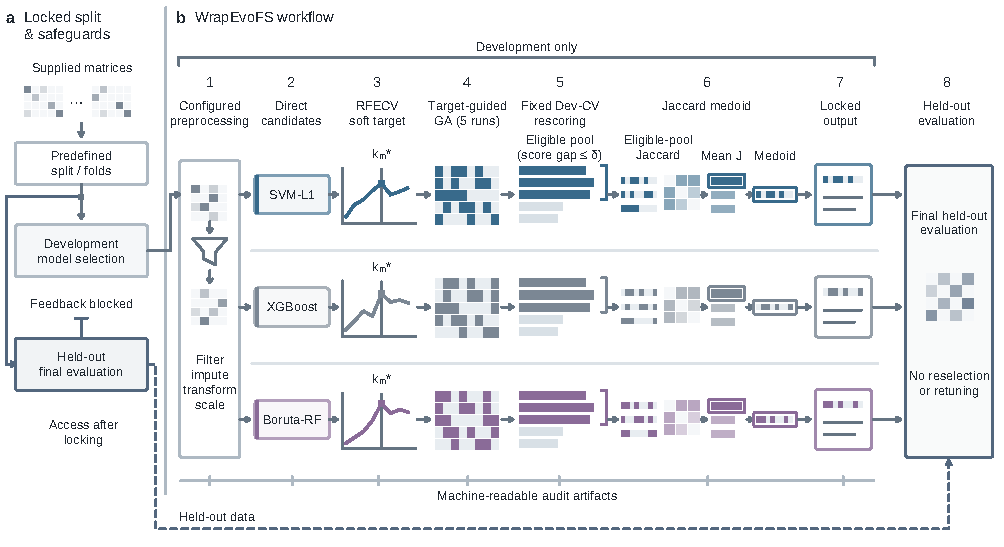
\includegraphics[width=170mm]{figures/figure_1_v19_figma.pdf}
\caption{\textbf{Development-only feature selection and representative locking.}
a) Predefined partitions separate development-only selection from held-out evaluation. The blocked return path indicates that held-out outcomes do not inform selection or tuning.
b) Configured preprocessing (1) and Direct screening (2) define three branch-specific feature universes: SVM-L1, XGBoost and Boruta-RF. These labels identify screening branches. Recursive feature elimination with cross-validation (RFECV; 3) supplies a soft target count $k_m^*$, and five target-guided genetic algorithm (GA) runs (4) generate candidate sets within each branch. Fixed development cross-validation (Dev-CV; 5) rescores candidates and identifies the regret-eligible pool within the allowed score gap $\delta$. Within that pool, pairwise Jaccard similarities determine the mean overlap of each candidate with the other eligible candidates (6); diagonal self-comparisons are excluded. The highlighted medoid is one existing candidate with maximal mean overlap, not a union or newly generated consensus mask. Its output is locked (7) before held-out evaluation (8). The final estimator is fitted on development data after locking, with no held-out-driven reselection or retuning. The solid lower trace denotes machine-readable audit artifacts; the dashed route denotes held-out data accessed only after locking. Blue, slate and plum consistently identify the three screening branches. Curves, score bars, matrices and masks are schematic examples, not empirical measurements; the three eligible candidates shown are illustrative, and pool size is not fixed at three.}
\label{fig:workflow}
\end{figure}
\FloatBarrier

The empirical designs distinguish development-only selection, fully nested assessment, and one-time post-freeze held-out evaluation (\Cref{tab:main1}).

{
\footnotesize
\renewcommand{\arraystretch}{1.00}
\setlength{\tabcolsep}{2.2pt}
\begin{longtable}{@{}>{\raggedright\arraybackslash}p{0.1326\linewidth}>{\raggedright\arraybackslash}p{0.1486\linewidth}>{\raggedright\arraybackslash}p{0.1968\linewidth}>{\centering\arraybackslash}p{0.1326\linewidth}>{\raggedright\arraybackslash}p{0.1547\linewidth}>{\centering\arraybackslash}p{0.1747\linewidth}@{}}
\caption{Empirical datasets, evaluation designs, outcome composition, and predictor inventories}\label{tab:main1}\\
\toprule
\bfseries Dataset & \bfseries Endpoint & \bfseries Evaluation design & \bfseries Participants & \bfseries Outcome composition & \bfseries Input predictors \\
\midrule
\endfirsthead
\multicolumn{6}{l}{\footnotesize\itshape \tablename~\thetable\ (continued)}\\
\toprule
\bfseries Dataset & \bfseries Endpoint & \bfseries Evaluation design & \bfseries Participants & \bfseries Outcome composition & \bfseries Input predictors \\
\midrule
\endhead
\bottomrule
\endfoot
ADNI-derived multi-omics & CN / MCI / dementia & Fixed stratified 80:20 development/held-out split & 665 total; 532 development; 133 held-out & Development 103/187/242; held-out 26/47/60 & 7,411 processed; 7,002 proteomic; 409 metabolomic \\
AMP-AD multicenter multi-omics & Ordered bScore: Low / Moderate / High & Four fixed leave-one-center-out folds & 527; every participant held out once per prespecified configuration & 111 / 156 / 260 overall; center-specific counts archived & 13,136 supplied before fold filtering; 11,748 frontal proteomic; 1,388 metabolomic \\
CGGA all-glioma gene expression & MGMT methylated / unmethylated & Fixed stratified 70:30 development/held-out split & 306 total; 214 development; 92 held-out & Development 110/104; held-out 47/45 & 24,326 gene-expression predictors \\
TCGA GBM/LGG multi-omics & Historical histological type: GBM / astrocytoma / oligodendroglioma / oligoastrocytoma & Two stratified five-fold outer-CV repeats & 491; every participant held out once per repeat & 66 / 147 / 165 / 113 & 25,118 supplied; 20,118 RNA-seq; 5,000 cleaned SCNV \\
Private T1ce radiomics & MGMT unmethylated / methylated & Fixed stratified 70:30 development/held-out split; two feature spaces share participants & 197 total; 137 development; 60 held-out & Development 81/56; held-out 36/24 & 1,781 full-space; 1,346 label-independent perturbation-filtered \\
\end{longtable}
}


\FloatBarrier
\section{Results}

\subsection{Representative locking balances score and feature overlap}

Representative locking addresses the choice of one signature from a bank of near-scoring alternatives. Candidates within the declared development-score allowance form the eligible pool; its medoid is the existing candidate with the greatest average Jaccard overlap with the other eligible sets.

The four locking rules answer distinct decision questions (\Cref{tab:locking-rule-distinction}). The highest-locking-score candidate guarantees zero empirical regret but does not optimize representativeness. The unrestricted full-bank medoid optimizes full-bank representativeness without a nontrivial score-gap guarantee, whereas the top-three medoid substitutes a rank cutoff for a metric-scale constraint. The regret-constrained medoid first enforces eligibility and only then optimizes within-pool mean Jaccard.

\begin{table}[!htbp]
\centering
\caption{Decision rules for selecting one feature set from a finite stochastic candidate bank.}
\label{tab:locking-rule-distinction}
\footnotesize
\renewcommand{\arraystretch}{1.12}
\setlength{\tabcolsep}{3pt}
\begin{tabularx}{\linewidth}{@{}>{\raggedright\arraybackslash}p{0.16\linewidth}>{\raggedright\arraybackslash}p{0.18\linewidth}>{\raggedright\arraybackslash}p{0.23\linewidth}>{\raggedright\arraybackslash}p{0.18\linewidth}>{\raggedright\arraybackslash}X@{}}
\toprule
\bfseries Rule & \bfseries Admissible pool & \bfseries Primary decision & \bfseries Empirical-regret guarantee & \bfseries Representativeness target \\
\midrule
Highest-locking-score candidate & Full bank & Maximize locking score & Zero & Not explicitly optimized \\
Top-three medoid & Three highest-ranked candidates & Maximize mean Jaccard within the rank-restricted pool & No metric-scale bound & Rank-restricted pool \\
Unrestricted full-bank medoid & Full bank & Maximize mean Jaccard within the full bank & No nontrivial bound & Full candidate bank \\
Regret-constrained medoid & $E_{\delta}=\{r:R_r=L_{\mathrm{best}}-L_r\leq\delta\}$ & Maximize mean Jaccard within $E_{\delta}$ & $R_{\mathrm{selected}}\leq\delta$ & Strict regret-eligible pool \\
\bottomrule
\end{tabularx}
\end{table}

\FloatBarrier

\subsection{Fully nested assessment of compression and performance}

The fully nested benchmark quantified the performance--compression trade-offs of compact, traceable signatures across three screening branches under a fixed reference allowance of \(\delta=0.01\).

The TCGA GBM/LGG benchmark moved the complete selection pipeline inside two repeated five-fold outer-CV partitions for 491 participants. The design yielded 150 candidates in 30 banks without outer-test access during selection or locking. At \(\delta=0.01\), the top-three medoid exceeded the allowed development-score gap in 5 banks (maximum 0.0236), and the unrestricted medoid exceeded it in 14 (maximum 0.0387); the regret-constrained medoid had no exceedance (maximum 0.00978; Supplementary Table~S31a). Highest-score selection also has zero gap, but does not optimize candidate overlap. The regret-constrained medoid differed from that candidate in 11 banks, and every change increased eligible-pool mean Jaccard (median gain 0.0429; \Cref{fig:tcga-nested}a,b; Supplementary Fig.~S5).

Mean within-bank pairwise Jaccard among the five GA candidates was 0.115, compared descriptively with 0.103 expected for uniformly sampled subsets with the same bank-specific universe and candidate sizes; mean Jaccard among locked signatures across outer folds was 0.0357 (\Cref{fig:tcga-nested}c). Across outer partitions, similar signature size did not imply similar feature identity: 42 of 60 paired locked signatures had cardinality similarity at least 0.9, yet 33 of those 42 pairs had feature-set Jaccard at most 0.05 (\Cref{fig:tcga-nested}d). Supplementary Fig.~S6 reports chance-corrected candidate agreement, all dependent outer-fold pairwise similarities, and RNA/SCNV composition. These descriptive measures distinguish stochastic-search agreement from participant-partition sensitivity within this cohort.

The locked signatures reduced Direct feature counts by 80--82\%, retaining means of 14.6, 20.0, and 18.0 features from 81, 100, and 100 in the SVM-L1, XGBoost, and Boruta-RF branches; RFECV-only retained 12.7, 19.4, and 8.8 features. These reductions describe the complete pipeline. Mean repeated out-of-fold (OOF) macro one-vs-rest area under the receiver operating characteristic curve (AUROC) was 0.827, 0.827, and 0.828, compared with Direct values of 0.840, 0.831, and 0.843. Paired locked-minus-Direct differences were $-0.0132$ (95\% CI $-0.0242$ to $-0.0031$), $-0.0043$ ($-0.0144$ to 0.0063), and $-0.0156$ ($-0.0249$ to $-0.0062$), respectively (\Cref{fig:tcga-benchmark}a; Supplementary Table~S31b). Corresponding differences from RFECV-only were $-0.0108$ ($-0.0259$ to 0.0035), 0.0012 ($-0.0113$ to 0.0134), and 0.0054 ($-0.0125$ to 0.0225); all three RFECV-only intervals included zero.

Within the same candidate banks, paired outer-test comparisons isolated the choice of locking rule (\Cref{fig:tcga-benchmark}b). Regret-constrained-minus-highest-score AUROC differences were $-0.0058$, $-0.0050$, and $+0.0029$ for SVM-L1, XGBoost, and Boruta-RF; all three 95\% intervals included zero. Against the unrestricted medoid, XGBoost increased by 0.0090 (95\% CI 0.0001 to 0.0176), while the other two intervals included zero. All nine rule-level contrasts are shown together, separating the representative-locking decision from the upstream feature-selection pipeline.

A retrospective selector-layer analysis under a frozen protocol compared the signatures with nested multinomial Elastic Net, subsampling stability selection, and random banks within identical post-Direct outer-training universes (\Cref{fig:tcga-benchmark}c,d; Supplementary Figs.~S7--S8; Supplementary Table~S6). Native supports were the prespecified primary selector comparators. Native Elastic Net retained means of 60--77 features and had higher AUROC in SVM-L1 and Boruta-RF, with locked-minus-native differences of $-0.0146$ (95\% CI $-0.0251$ to $-0.0045$) and $-0.0108$ ($-0.0199$ to $-0.0012$). Native stability selection retained 58 features in SVM-L1, with a difference of $-0.0136$ ($-0.0245$ to $-0.0029$). At matched cardinality, SVM-L1 WrapEvoFS exceeded Elastic Net by 0.0176 (0.0008 to 0.0341) and stability selection by 0.0261 (0.0082 to 0.0434). XGBoost differences were $-0.0017$ ($-0.0146$ to 0.0111) and $-0.0015$ ($-0.0136$ to 0.0105). Boruta-RF differences were $-0.0109$ ($-0.0236$ to 0.0024) and $-0.0128$ ($-0.0260$ to 0.0012). Across five random-bank replicates per condition (150 banks in total), mean locked-minus-random AUROC differences were $-0.0018$, $+0.0102$, and $-0.0043$. These controls match candidate count and locking-evaluation budget, not full GA compute. Together, the comparisons quantify branch-specific choices between predictive performance and signature size.

A retrospective diagnostic evaluated all 150 saved candidates with the original common final-estimator seeds, reproducing the 120 existing candidate-based rule predictions to numerical precision. The mean within-bank range of outer-test AUROC was 0.0309. In 200 class-stratified half-splits of each outer-test bank, selecting the best run on one half and evaluating that run on the other gave mean AUROCs of 0.8493 on the selection half and 0.8239 on the opposite half, averaging both directions (difference 0.0253; Supplementary Table~S31c). This fixed-bank diagnostic quantifies the scale of outcome-informed run-selection optimism in these small evaluation halves. It supports specifying a rule before evaluation; it does not distinguish the proposed medoid from other development-only rules on that principle.

\begin{figure}[H]
\centering
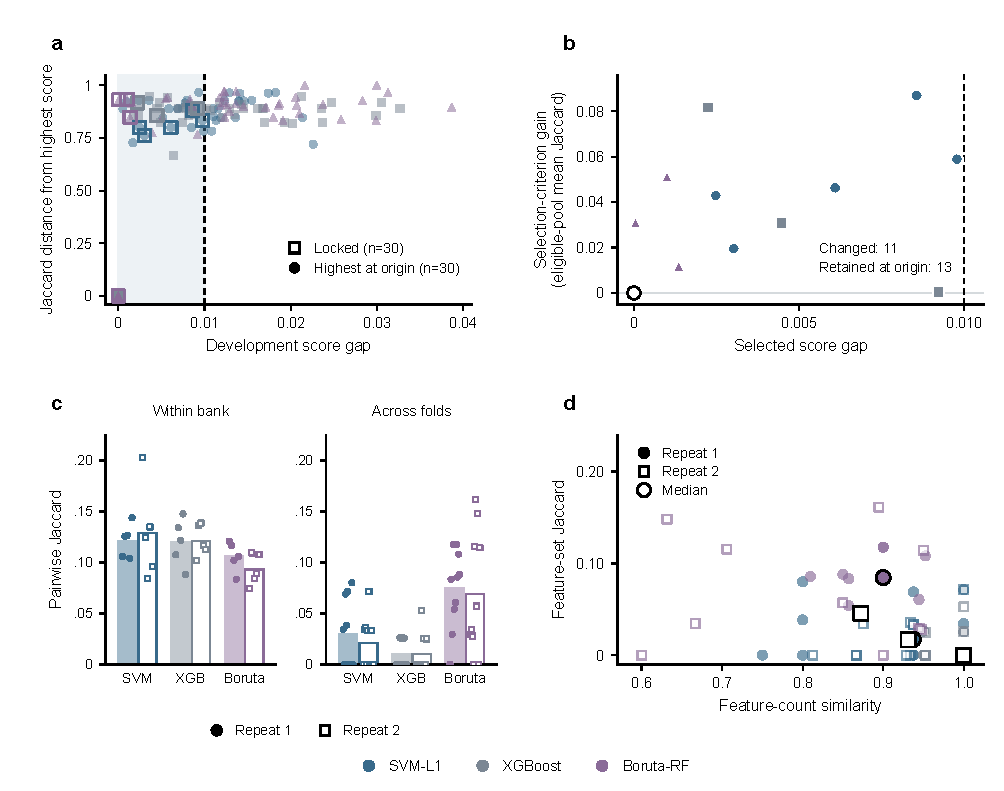
\includegraphics[width=170mm]{figures/figure_4_strengthened.pdf}
\caption{\textbf{Representative locking and feature-set agreement in the fully nested TCGA analysis.}
Two five-fold outer-CV repeats across three Direct branches yield 30 banks of five candidates from 491 participants.
a) Candidate development-score gaps and Jaccard distances from the highest-scoring candidate. The shaded region and dashed line mark eligibility at $\delta=0.01$; open squares denote locked medoids. The 30 highest-scoring candidates coincide at the origin.
b) Selected-minus-highest-scoring mean Jaccard overlap within the 24 nonsingleton eligible pools. Eleven changed selections are shown individually; 13 retained highest-scoring candidates coincide at the origin. Six singleton pools are excluded because the gain is undefined. This is the optimized within-pool selection criterion.
c) Distinct sources of feature-set variation are shown separately on a common scale. Within-bank points are the five outer-fold bank means per branch and repeat; each bank mean averages the ten pairwise overlaps among all five GA candidates. Across-fold points are the ten dependent pairs of locked feature sets per branch and repeat. Bars show the corresponding descriptive means; all 30 bank means and 60 outer-fold pair values are retained. No inferential intervals are estimated from these dependent comparisons.
d) Feature-count similarity, $\min(k_1,k_2)/\max(k_1,k_2)$, versus feature-set Jaccard for 60 dependent outer-fold pairs. Larger, black-outlined markers show coordinate-wise branch-repeat medians.
Colors identify Direct branches. In c and d, filled circles and open squares identify repeats 1 and 2; bars in c use filled and open forms for the same repeats. SVM and XGB abbreviate SVM-L1 and XGBoost.
Outer-test data were excluded from selection and locking. Overlap measures describe search and participant-partition sensitivity, not independent biomarker replication.}
\label{fig:tcga-nested}
\end{figure}

\begin{figure}[H]
\centering
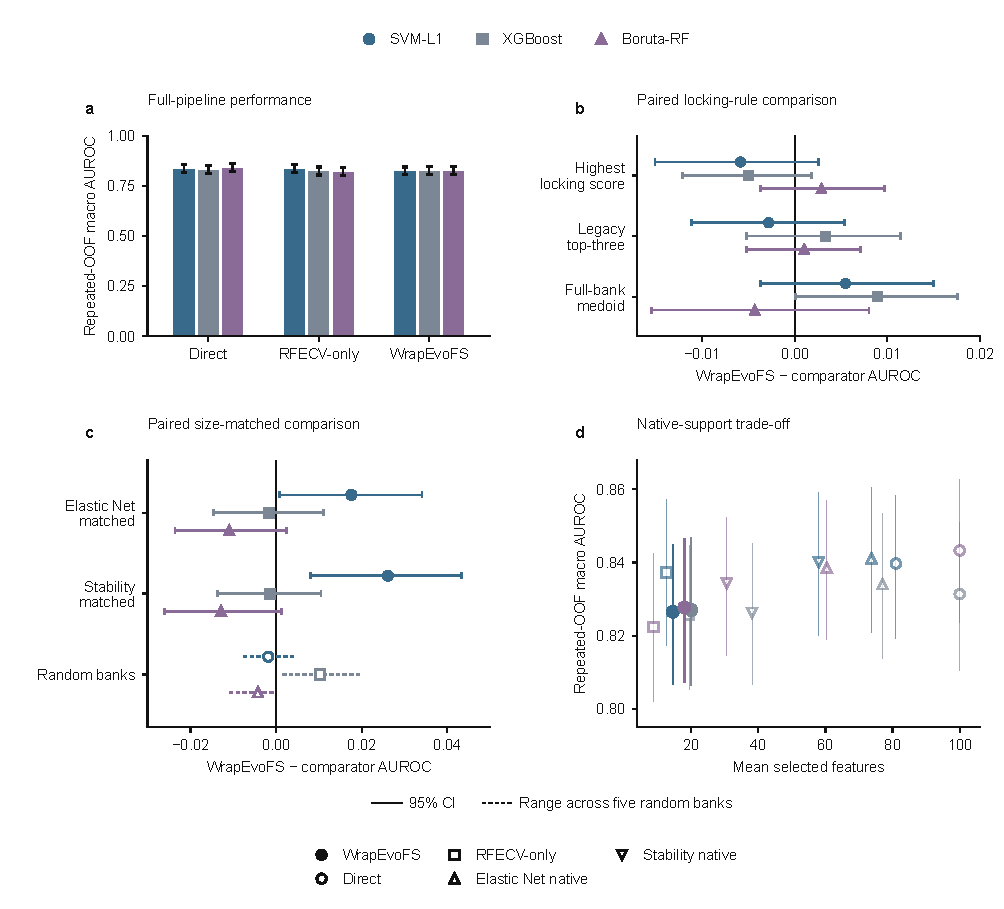
\includegraphics[width=170mm]{figures/figure_3_strengthened.pdf}
\caption{\textbf{Representative locking and predictive trade-offs in the nested TCGA benchmark.} Analyses use 491 participants, two stratified five-fold outer-CV repeats, training-only selection, and a common final random forest. a) Mean repeat-specific out-of-fold macro one-vs-rest AUROC for Direct, RFECV-only, and WrapEvoFS. b) Paired WrapEvoFS-minus-comparator AUROC differences for three locking rules applied to the same candidate banks: highest locking score, top-three medoid, and unrestricted full-bank medoid. c) Corresponding differences against cardinality-matched Elastic Net and stability rankings and five random-bank replicates. Colors and, in b,c, marker shapes identify Direct branches. Solid intervals are nominal 95\% confidence intervals from 2,000 participant-clustered, class-stratified bootstrap resamples retaining both repeat predictions. Dashed intervals in c are observed ranges across five random banks. d) Mean feature count versus AUROC, including native Elastic Net and stability supports; marker shape identifies the selector, filled circles identify WrapEvoFS, and vertical lines show AUROC intervals. Compression is measured relative to Direct; matched selector comparisons share its branch-specific feature universe. Confidence intervals are conditional on fitted models and realized partitions.}
\label{fig:tcga-benchmark}
\end{figure}

\subsection{Tolerance sensitivity and development-only calibration}

The tolerance controlled the number of alternatives considered and exposed how selection responds to development-score variation.

Original five-candidate banks from 36 AMP-AD center--branch--cap conditions and six CGGA branch--guidance conditions provided a complementary development-only sensitivity analysis. Increasing absolute tolerance enlarged their strict eligible pools (Supplementary Fig.~S4). At the prespecified \(\delta=0.01\), the locked candidate's mean Jaccard with the other four bank members had medians of 0.204 and 0.424, respectively. The original audits normalized Nogueira's coefficient over the observed union of the five saved masks; the corresponding medians were $-0.063$ and 0.076 (Supplementary Methods S1.3). These are descriptive fixed-bank agreement summaries, with the normalization retained explicitly.

A paired development-fold weighting analysis used 54 complete five-candidate banks: the 30 TCGA banks above and 24 additional AMP-AD banks spanning four centers, three screening branches, and two feature-count caps (Supplementary Fig.~S29; Supplementary Table~S29). The latter used an untruncated size-penalized GA objective, termed the corrected-objective configuration; its technical verification appears in \Cref{sec:objective-verification}. Leave-one-fold-out weighting retained the original regret-constrained signature in 75.2\% of cases, versus 79.3\% for highest-score selection. Exhaustive fold-bootstrap weighting gave corresponding probabilities of 62.5\% and 65.4\%. The unrestricted medoid retained its signature throughout because its geometry was fixed, but exceeded the 0.01 score-gap threshold in 55.8\% of fold-bootstrap cases; the top-three medoid exceeded it in 21.8\%. These profiles distinguish decision sensitivity from score-gap control using the same candidates and score perturbations.

An exploratory repeated-search extension used 240 additional GA runs on one fixed TCGA outer-training partition (392 participants), with 80 candidates organized into 16 disjoint five-candidate banks per branch. Calibration selected the allowance using development scores and cross-bank feature overlap alone. Exact enumeration of observed within-bank score gaps replaced the seven-point numerical grid of an earlier calibration pilot; 65 breakpoints were evaluated per branch and scoring scheme. With the original candidate-seed scorer, the selected allowances were 0.009519, 0.007563, and 0.008453 for SVM-L1, XGBoost, and Boruta-RF (Supplementary Methods S1.15; Supplementary Table~S32a).

Across branches, breakpoint calibration gave fitted-bank Jaccard of 0.1318, compared with 0.1298 for grid calibration, 0.1261 for fixed 0.01, and 0.1220 for highest-score selection. Mean signature-level AUROC on the same held-out 99 participants was 0.8461, 0.8474, 0.8463, and 0.8466, respectively. Breakpoint-minus-comparator differences were $-0.00130$ (simultaneous 95\% CI $-0.00311$ to 0.00050), $-0.00018$ ($-0.00207$ to 0.00171), and $-0.00050$ ($-0.00500$ to 0.00399). The increased overlap was the fitted calibration objective; these comparisons did not establish predictive superiority or improved reproducibility on new banks. The earlier grid-calibration check on separately reserved seed banks also did not establish superiority (Supplementary Table~S32b,c). The breakpoint extension was designed after earlier results were available and remains an exploratory internal analysis.

\subsection{Frozen selections undergo one-time multicenter evaluation}

The 24 additional AMP-AD signatures were fixed before paired assessment across four held-out centers under a common freeze-and-evaluate protocol.

After the 24 corrected-objective AMP-AD locks and the evaluation protocol were frozen, each signature was evaluated once in its corresponding held-out center without reselection or parameter changes (\Cref{fig:ampad-postfreeze}; Supplementary Fig.~S9; Supplementary Table~S7). Pooled differences ranged from $-0.0404$ to $+0.0480$ against RFECV-only and from $-0.0311$ to $+0.0176$ against the top-three medoid. Four of six RFECV-only contrasts and five of six top-three contrasts had 95\% intervals including zero. Of the three non-zero-crossing intervals, the two RFECV-only contrasts favored opposite directions across branches, whereas the single top-three contrast favored the top-three medoid. Because the masks and evaluation protocol were frozen before held-out outcome access, this analysis evaluates protocol adherence and center transport. The paired contrasts resolve branch- and cap-specific performance under this fixed evaluation protocol.

A fixed-center sensitivity distinguished pooled prediction ranking from average within-center performance (\Cref{fig:ampad-postfreeze}b,c; Supplementary Table~S30). For XGBoost/Small versus RFECV-only, the pooled difference of 0.0480 (95\% CI 0.0253 to 0.0704) corresponded to an equal-center mean difference of 0.0098 ($-0.0198$ to 0.0412). Conversely, Boruta-RF/Reference versus the top-three medoid had an equal-center difference of 0.0327 (0.0067 to 0.0597), while its pooled interval included zero. Reporting both summaries preserves the original pooled evaluation and identifies how center aggregation affects the comparison.

\begin{figure}[tbp]
\centering
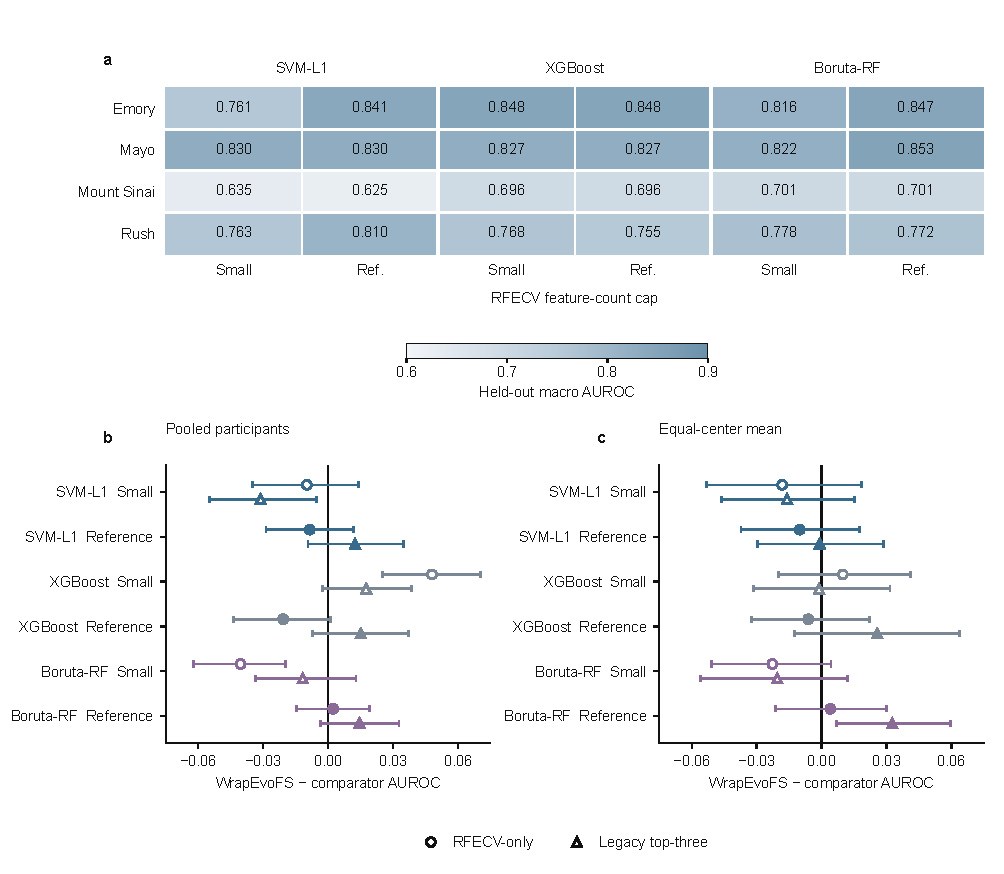
\includegraphics[width=170mm]{figures/figure_5_strengthened.pdf}
\caption{\textbf{Held-out-center performance and sensitivity to center weighting.} Frozen AMP-AD signatures were evaluated in Emory, Mayo, Mount Sinai, and Rush (80, 217, 52, and 178 participants, respectively). a) Macro one-vs-rest AUROC for all 24 center--branch--cap conditions. Cell shading and labels encode the same point estimate; Small and Ref. denote the Small and Reference RFECV feature-count caps. b) Paired AUROC differences between the corrected-objective, regret-constrained workflow and original RFECV-only or top-three signatures, calculated after concatenating predictions from the four held-out-center models. c) Post hoc sensitivity using the equally weighted mean of the four within-center AUROC differences. Panels b,c retain all 12 contrasts with the same axes and ordering. Circles denote RFECV-only and triangles the top-three medoid; open and filled symbols denote Small and Reference caps. Nominal 95\% paired percentile intervals use 2,000 common participant resamples within held-out-center-by-class strata (seed 42), conditional on these four centers and fitted models. Signatures and the original evaluation protocol were frozen before held-out outcome access; the corrected-versus-original comparison includes changes to candidate generation and locking.}
\label{fig:ampad-postfreeze}
\end{figure}

\subsection{Controlled candidate-bank locking simulation}

The simulation identified when representative locking improved hidden-utility selection: agreement had to carry useful signal relative to score noise.

A prespecified simulation isolated the locking layer under hidden utility across 4,995,000 synthetic banks (Supplementary Fig.~S28; Supplementary Table~S23). In all 54 primary scenarios combining aligned or competing topology with score-noise ratios of at least 1, the regret-constrained medoid had lower mean hidden-oracle regret than highest-score selection. The improvements were small and conditional on the simulated geometry. With noiseless scores, highest-score selection was preferable, and misleading consensus could increase loss. Across the complete primary $R=5$, $\delta=0.01$ grid, mean full-bank Jaccard increased from 0.424 to 0.446 relative to highest-score selection, while mean hidden-oracle regret was 0.00259 versus 0.00222; both lower oracle regret and higher representativeness occurred in 91 of 162 scenarios. Thus, the simulation explains the score-noise and consensus conditions under which a representative candidate can be useful, while retaining the complete primary trade-off.

\subsection{Objective flattening and corrected-objective verification}
\label{sec:objective-verification}

The corrected-objective configuration reduced aggregate deviation from the target feature count, with the largest reduction in the prespecified stress condition.

Eighteen of 36 original AMP-AD configurations triggered at least one zero-truncation warning; none of six original CGGA configurations did. The most severe condition was AMP-AD Rush/SVM-L1/Small: target \(k^*=3\), locked count 84, absolute deviation 81, four of five zero-valued run-best fitness, and 245 all-zero generations. This provides a concrete loss-of-ordering mechanism beyond the general observation that genetic search is variable (Supplementary Fig.~S1; Supplementary Tables~S1--S2).

The matched development-only comparison comprised 120 corrected-objective GA runs, compared with matched archived original banks, in 24 combinations of center, branch, and Small or Reference cap (\Cref{fig:updated-verification}; Supplementary Fig.~S2; Supplementary Tables~S1--S2). Aggregate absolute target deviation decreased from 216 to 137; the corrected-objective configuration was better in 12 conditions, unchanged in 6, and worse in 6. The prespecified Rush/SVM-L1/Small stress condition accounted for 56 of the 79 reduced deviation units; excluding it, deviation decreased from 135 to 112. Zero-truncation diagnostic generations decreased from 673 to 333 overall and from 428 to 267 without the stress condition. The corrected-run counts apply the legacy truncation rule diagnostically to the recorded populations; they are distinct from actual parent-sampling fallbacks, which were zero.

All 24 locked sets satisfied the prespecified tolerance of 0.01 for empirical regret, the development-score gap from the best candidate in the same bank; the maximum selected regret was 0.00835 (\Cref{fig:updated-verification}c). Corrected-objective-minus-original fixed locking-score differences had mean \(+0.00098\), median \(+0.00096\), and range \(-0.01319\) to \(+0.02389\); uniform parent-sampling fallbacks were zero. This comparison establishes configuration-level target fidelity and score-gap behavior; the cross-lock analysis separates the two stages. Held-out outcomes were accessed only after the protocol and all 24 selected masks were frozen.

The existing-artifact 2 by 2 cross-lock analysis separated candidate-bank and locking-rule effects (\Cref{fig:updated-verification}d; Supplementary Table~S3). Within 24 original-objective banks, the regret-constrained medoid changed 10 masks and reduced mean and maximum selected regret from 0.00261 and 0.02111 to 0.00060 and 0.00729, while total target deviation changed from 216 to 227. Within the 24 corrected-objective banks, it changed 8 masks and reduced mean and maximum regret from 0.00351 and 0.01525 to 0.00108 and 0.00835, while target deviation changed from 135 to 137. The two stages provide complementary controls: candidate generation determines target fidelity, while representative locking enforces the configured score-gap bound.

At \(\delta=0.01\), 2 of the 24 corrected-objective conditions had singleton eligible pools, 6 had two candidates, and 16 had at least three (Supplementary Table~S4). Unique Jaccard medoids determined 13 selections, higher locking score resolved 9, and singleton selection resolved 2; neither feature count nor the stable mask hash, a content-derived identifier used as the final tie-breaker, was needed. No exact duplicate mask occurred in the 48 complete banks, and all recovered Rush selections matched their archived and frozen-evaluation records.

\begin{figure}[tbp]
\centering
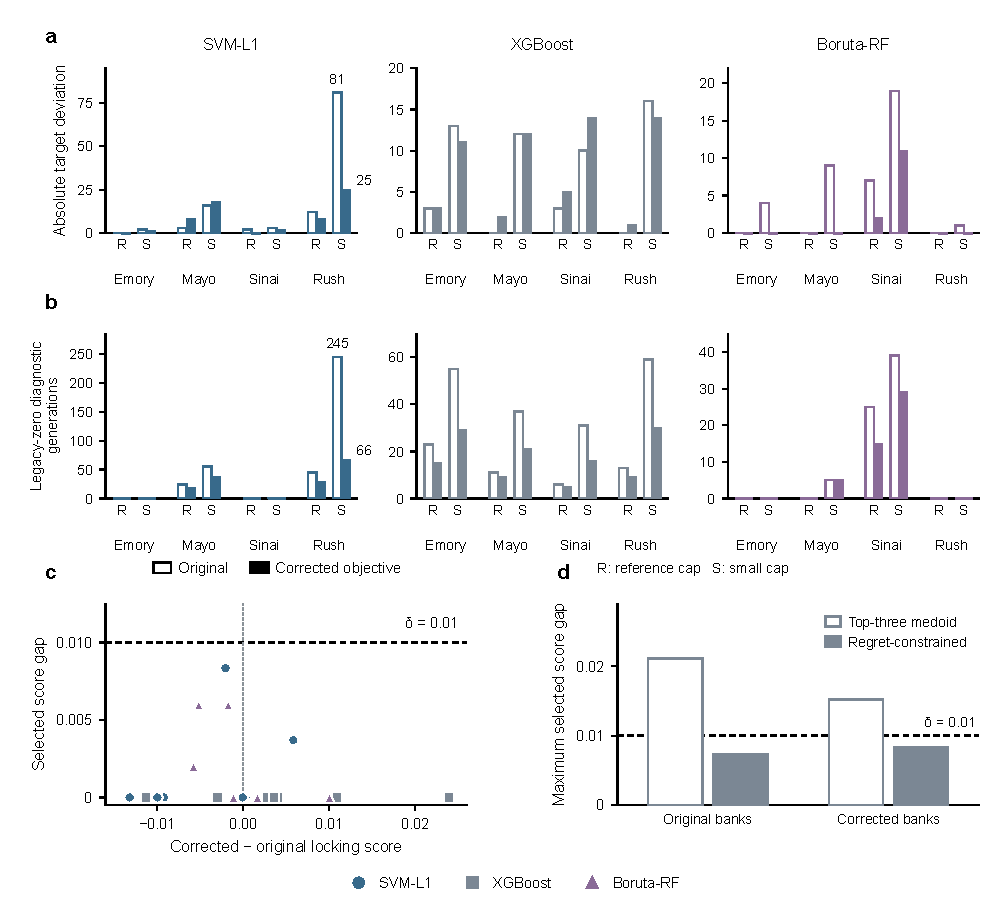
\includegraphics[width=170mm]{figures/figure_2.pdf}
\caption{\textbf{Corrected-objective search and score-constrained locking in the development-only comparison.}
The comparison includes 120 corrected-configuration GA runs (five per condition) and matched archived original banks across 24 center--branch--cap conditions.
a,b) Absolute deviation of the final locked mask from the RFECV target (a) and legacy-zero diagnostic generation counts summed across five runs per condition (b), with paired bars for every condition. Updated counts apply the legacy truncation rule diagnostically to corrected-search histories; actual uniform-sampling fallbacks were zero.
Columns identify branches; within each center, R and S denote reference and small caps. Sinai abbreviates Mount Sinai.
Open and filled bars denote original and corrected-objective values, respectively.
All bar axes start at zero; their explicitly labelled ranges differ by branch. No condition is omitted or repeated in an enlarged view. Numbers identify the prespecified Rush/SVM-L1/small-cap stress condition.
c) Corrected-minus-original development-CV locking score against the selected candidate's score gap from the best candidate. The dashed horizontal line marks the 0.01 tolerance.
d) Existing-artifact cross-lock comparison: each of the original and updated candidate-bank collections is locked with both the top-three and regret-constrained rules. Each bar is the maximum selected development-score gap across the same 24 conditions; the dashed line marks $\delta=0.01$. The regret-constrained bound follows from eligible-only selection. Pool-size and tie-path distributions remain in Supplementary Table~S4.
Candidate generation and locking both changed in a--c, whereas d applies both rules to each fixed bank collection. All summaries are descriptive; no held-out outcomes informed the comparison.}
\label{fig:updated-verification}
\end{figure}

\subsection{Archived and cross-modal analyses define empirical scope}

The additional cohorts demonstrate compression and downstream use across distinct feature modalities and evaluation designs.

Across 36 archived AMP-AD banks, retrospective regret-constrained re-locking compressed the corresponding Direct sets by a median 74.1\% (range 15.8\%--80.0\%); median empirical score gap was 0 and the maximum was 0.0091. Across six CGGA banks, median compression was 57.9\% (range 34.3\%--70.0\%), median gap was 0.00065, and maximum gap was 0.00355 (Supplementary Fig.~S3; Supplementary Table~S5). Recovery of the complete five-mask ADNI banks enabled the same audit without rerunning selection or accessing held-out outcomes. At absolute $\delta=0.01$, all three eligible pools were singletons and the selected empirical regret was zero. The rule retained the original top-three XGBoost selection but changed the SVM-L1 and Boruta-RF selections, for which the original top-three score gaps were 0.0140 and 0.0225, respectively (Supplementary Table~S8).

Archived original-configuration demonstrations remain fully reported in the Supplement. ADNI locked signatures reduced Direct counts by 44\%--70\%, but all nine primary paired held-out intervals crossed zero (Supplementary Figs.~S10--S12; Supplementary Tables~S8--S9). Original AMP-AD effects varied by center, branch, cap, metric, and comparator (Supplementary Figs.~S13--S14; Supplementary Tables~S10--S12). CGGA showed 54\%--73\% compression, target-size control in the archived guidance ablation, and variable feature agreement without a uniform predictive advantage (Supplementary Figs.~S15--S19; Supplementary Tables~S13--S18).

The VGH brain-tumour radiomics cohort (UBC REB H20-02354, ``Brain Tumor Image Analysis'') provided a supplementary internal test in a distinct feature modality. The same 197 MGMT-linked participants were analyzed under a frozen 137/60 development/held-out split in full and label-independent perturbation-filtered feature spaces (Supplementary Fig.~S20). All six locks had zero empirical development-CV regret at \(\delta=0.01\), with 10.0\%--81.0\% compression relative to Direct sets (median 75.6\%). Paired held-out locked-minus-Direct AUROC estimates ranged from \(-0.007\) to 0.069, and all 95\% intervals included zero (Supplementary Table~S19). This analysis broadens the tested modality but reuses participants across feature spaces, relies on unadjudicated automatic regions, and remains internal.

\subsection{Secondary held-out trade-offs and interoperability}

A locked feature set supplied a reproducible candidate set for several downstream analysis methods.

Secondary tuned-model, computational, random-subset, and Elastic Net analyses are reported in Supplementary Figs.~S21--S23 and Supplementary Table~S16. Bayesian, STABL, and BLiP analyses used the locked ADNI outputs as reproducible downstream candidate sets without reopening held-out-informed selection (Supplementary Figs.~S24--S27; Supplementary Tables~S20--S22). Five of eight features selected by training-only STABL overlapped the 78-feature WrapEvoFS locked-signature union, yielding an 81-feature candidate set for restricted downstream analyses (Supplementary Figs.~S26--S27; Supplementary Table~S21). The corresponding 81-feature restricted Laplace Bayesian model yielded a held-out macro one-vs-rest AUROC of 0.803 (95\% CI 0.744--0.856), compared descriptively with 0.780 for the 7,411-feature Bayesian reference, for which a confidence interval was unavailable (Supplementary Figs.~S24--S25 and S27; Supplementary Tables~S20--S22). Directions varied by method, and agreement is not independent replication because the analyses reuse the same development boundary.

\FloatBarrier
\section{Discussion}

WrapEvoFS provides a concrete decision procedure for retaining one compact signature from repeated stochastic searches. An explicit empirical score-gap allowance limits the alternatives, and feature overlap determines the representative candidate within that pool. The allowance may be declared directly or calibrated from development data. In the nested TCGA benchmark, the workflow reduced Direct feature counts by 80--82\%, retained 15--20 features on average, and changed 11 of 30 highest-score selections. The observed gap exceedances of rank-based and unrestricted medoids show why a metric-scale constraint matters when representativeness is a selection goal. The accompanying AUROC comparisons make the predictive cost of compression explicit across branches.

RFECV-guided genetic search separates a data-derived size reference from feature identity. In the original CGGA ablation, guidance narrowed five-run feature-count ranges from 16--23 to 15--16 (SVM-L1), 33--39 to 19--21 (XGBoost), and 10--14 to nine in every run (Boruta-RF; Supplementary Fig.~S17b). Pipeline comparison and locking-rule comparison answer different questions: RFECV, Elastic Net, and stability selection generate feature sets, whereas locking rules choose among a supplied stochastic bank. Native and matched-cardinality controls describe the resulting choices between performance and measurement count; no selector dominated every branch on both.

The procedure is useful when repeated searches have already produced alternative compact signatures and one must be fixed for a downstream assay, model, or follow-up analysis. It preserves an existing candidate and its provenance rather than constructing a larger union. The random-bank controls demonstrate that the same rule can act after candidate generation independently of GA exploration. The outcome-informed run-selection diagnostic supports fixing a rule before inspecting evaluation results. Its medoid-specific contribution is to turn feature overlap into an explicit, deterministic selection preference among candidates that meet the score budget. The simulation further identifies a setting where overlap can help resolve noisy score rankings: candidate agreement must contain information about useful alternatives.

Development-only calibration makes the operating allowance a recorded choice adapted to the available candidates. Enumerating score-gap breakpoints removes the need to privilege a numerical value such as 0.01 or to construct an arbitrary search grid. The 240-run study demonstrates this finite calibration procedure, while its fitted overlap gains and uncertain held-out contrasts delimit what has been established. Calibration and representative locking remain separate: calibration chooses an allowance across development banks, whereas locking chooses an existing candidate within each eligible pool.

The score-gap bound is finite-bank and empirical. Five seeds sparsely sample a search, and TCGA feature identities remained sensitive to participant partitions. Except in the fully nested TCGA design, preprocessing and Direct screening preceded locking-score folds, with adaptive fold reuse. The selector-layer comparison was retrospective and conditional on post-Direct universes in one internal cohort. The calibration extension reused one fixed participant partition; fitted-bank overlap is not unseen-seed or participant-resampling validation, and its development-score filter is not a guarantee of held-out performance. The radiomics analysis used automatic, non-adjudicated regions, and held-out-center effects were heterogeneous. The half-split diagnostic is conditional on fixed candidates, fitted models, and small evaluation halves; it is not an external estimate of selection bias or a unique advantage of medoid locking. Broader cohorts and participant-resampling studies are needed to establish transportability and biomarker reproducibility.

WrapEvoFS makes the final choice among stochastic feature sets explicit and reproducible. Its practical output is one compact, traceable signature selected under a declared or development-calibrated score allowance, together with the information needed to assess compression, predictive trade-offs, and feature-identity sensitivity.

\FloatBarrier
\section{Methods}

\subsection{Overall analytical workflow and leakage boundary}

\Cref{fig:workflow} separates development-only selection from one-time held-out evaluation. Preprocessing and Direct screening precede RFECV target estimation; five genetic searches per branch generate retained run-best subsets that a common development-CV evaluator rescores. A declared or development-calibrated tolerance defines the regret-eligible pool, whose Jaccard medoid is locked under deterministic tie-breaking. In the primary workflow, held-out outcomes cannot determine the strategy, tolerance, objective, metric, tie rule, or selected run, and trigger no reselection. Complete pseudocode and executable settings are provided in the Supplementary Methods and Supplementary Table~S24.

\subsection{RFECV target and primary estimands}

For each Direct branch (SVM-L1, XGBoost, or Boruta-RF) \citep{ref10,ref11,ref13}, RFECV follows a recursive elimination path on development folds and supplies a soft target: the smallest feature count attaining the best mean score among counts allowed by the configured cap. Compression is the fraction of Direct features removed by a selected set.

Let $F_r$ be the feature set of retained candidate $r$ in a bank of $R$ candidates. All candidates are evaluated on the same $K_L$ development folds using a fixed-specification random forest \citep{ref14} and a metric oriented so that larger values are better. If $s^L_{r\ell}$ is candidate $r$'s score on validation fold $\ell$, its locking score $L_r$, empirical regret $R_r$, and eligible pool $E_\delta$ are

\begin{equation}
L_r=K_L^{-1}\sum_{\ell=1}^{K_L}s^{L}_{r\ell},\qquad
R_r=\max_{1\leq j\leq R}L_j-L_r,\qquad
E_\delta=\{r:R_r\leq\delta\}.
\label{eq:regret-eligibility}
\end{equation}

Here $\delta\geq0$ is an explicit absolute development-score allowance, and $E_\delta$ contains candidate indices. Its value may be declared directly or obtained by a specified development-only calibration procedure; the held-out score is not an input to that procedure. Each fold score is obtained by fitting on the remaining folds and scoring the validation fold. All candidates share the fold partition, metric, and estimator specification; run-specific estimator seeds remain in the audit record. The search-stage metric may differ from the locking metric: search generates candidates, whereas the common locking evaluator compares them. Run-to-run agreement is summarized by pairwise Jaccard overlap, the selected candidate's mean overlap, and the chance-corrected Nogueira coefficient only when a complete run-by-feature matrix exists \citep{ref36}. These quantities describe stochastic agreement on one fixed development sample, not biomarker stability under participant resampling. Held-out performance differences are secondary and are calculated only after locking. Full notation for RFECV targeting, compression, locking scores, and held-out contrasts is provided in Supplementary Methods, Section~S1.2.

\subsection{Legacy-compatible and corrected genetic objectives}

A nonempty binary chromosome $\mathbf z$ represents feature set $F_m(\mathbf z)$ in Direct branch $m$. Let $\overline S_{G,m}(\mathbf z;\xi)$ be its mean search-stage score across fixed development folds with recorded seed $\xi$, $k_m^\ast$ the RFECV target, and $\lambda$ the penalty per feature of absolute target deviation. The penalized objective and its legacy-compatible transformation are

\begin{equation}
\begin{aligned}
Q_m(\mathbf z;\xi)&=\overline S_{G,m}(\mathbf z;\xi)-\lambda\left|\,|F_m(\mathbf z)|-k_m^\ast\,\right|,\\
\Phi_m^{\mathrm{legacy}}(\mathbf z;\xi)&=\max\{0,Q_m(\mathbf z;\xi)\}.
\end{aligned}
\label{eq:objective-comparison}
\end{equation}

Zero truncation makes distinct negative objectives indistinguishable. The corrected mode therefore uses $Q_m$ directly for reporting, ranking, elite selection, and run-best updating. A nonnegative shift is applied only to proportional parent-sampling weights and preserves the ordering of finite objectives. Uniform parent sampling is recorded when finite scores cannot define valid weights; empty chromosomes are prohibited. These scoring folds evaluate a frozen development-derived feature matrix: preprocessing and Direct screening are not refitted within each search-scoring fold. The package records zero-truncation, target-deviation, sampling-fallback, objective-diversity, and mask-diversity diagnostics. Fold-level definitions, sampling probabilities, and edge-case rules are provided in Supplementary Methods, Section~S1.2.

\Needspace{12\baselineskip}
\subsection{Regret-constrained medoid locking}

The eligible pool in \Cref{eq:regret-eligibility} is never expanded with a candidate outside the declared threshold. Because a highest-scoring candidate has zero regret, the pool is nonempty. If it contains one candidate, that candidate is selected. Otherwise, each eligible candidate's mean Jaccard similarity, defined as its average feature overlap with the other eligible candidates, is

\begin{equation}
\overline J_r=\frac{1}{|E_\delta|-1}\sum_{\substack{s\in E_\delta\\s\ne r}}
\frac{|F_r\cap F_s|}{|F_r\cup F_s|},
\label{eq:eligible-medoid}
\end{equation}

The candidate with the largest mean similarity is the eligible-pool Jaccard medoid. Remaining ties are resolved, in order, by higher locking score, fewer features, and a lexicographically smaller stable mask hash. The hash resolves otherwise identical selection criteria deterministically and is not a scientific score. Exact duplicate candidates retain their multiplicity as voting candidates, and source-run provenance is used only after the scientific feature set has been selected.

Selection is restricted to the eligible pool, so the output always satisfies the declared empirical score-gap tolerance. At zero tolerance, only highest-scoring candidates are eligible; tied maxima still undergo medoid selection. If the tolerance includes every candidate, the rule becomes the full-bank medoid. These guarantees concern the configured empirical development-CV score gap, not expected predictive risk, generalization error, or statistical uncertainty. Complete propositions, proofs, duplicate-policy details, and implementation correspondence are given in the Supplementary Methods and Supplementary Table~S25.

With \(R\) retained candidates, \(E\) eligible candidates, canonical-universe size \(p\), and average selected-set size \(s\), the package's dense-mask, sparse-Jaccard implementation has expected time \(O(Rp+E^2s+R\log R)\) and memory \(O(Rp+E^2)\). For the present \(R=5\) design, at most 10 unordered eligible pairs are compared; this use case does not establish large-bank scalability. Detailed representation-specific derivations are in the Supplementary Methods.

The reported nested TCGA and corrected-objective AMP-AD reference analyses used prespecified absolute \(\delta=0.01\) as a development-score budget for representative selection. This is a recorded reference setting rather than a universal default required by the locking rule. With macro AUROC as the locking metric, a candidate can exchange at most one percentage point of mean development-CV AUROC for greater eligible-pool feature overlap. This gives the score--representativeness trade-off an explicit metric-scale allowance; it does not bound held-out loss or define an optimal or clinical noninferiority margin. For scale, the 150 TCGA candidates had mean fold-based score SE 0.0109 in a retrospective descriptive check. This check did not determine \(\delta\) and is not a paired one-standard-error threshold. Development-only sensitivity evaluates 0, 0.005, 0.01, 0.02, and a best-run-SE-scaled threshold where fold vectors exist; the scaled sensitivity stops when the required vectors are absent.

For paired score sensitivity, the saved fold scores in all 54 TCGA and corrected-objective AMP-AD banks were reweighted without fitting new models or accessing held-out outcomes. We used five leave-one-fold-out vectors and all 126 five-fold bootstrap count vectors, weighted by their multinomial probabilities over 3,125 ordered resamples. All four locking rules received identical weights within each bank; summaries weighted banks equally. The fixed-bank protocol, provenance checks, and full distributions are reported in Supplementary Fig.~S29 and Table~S29.

\subsection{Development-only calibration of the score allowance}

The exploratory calibration study reused the first TCGA outer-training partition and generated 80 new candidates per branch using four 20-seed collections, the untruncated objective, and the recorded CPU implementation. Consecutive, nonoverlapping five-run blocks formed 16 calibration banks per branch. A candidate allowance was retained when its mean selected development score was at least the highest-score policy's mean minus one fold-based standard error. This standard error was calculated across five fold scores after averaging scores over banks. Among retained allowances, calibration maximized mean pairwise Jaccard between the bank-level signatures, resolving ties by higher mean development score and then smaller allowance. Zero allowance was included. This one-SE-style filter is a training heuristic, not a noninferiority test or performance guarantee.

The earlier calibration pilot searched seven numerical allowances. The breakpoint extension instead enumerated zero and all distinct gaps between candidates and their bank's best development score. Eligible pools and deterministic selections are constant between successive gaps, so this finite enumeration covers all possible selection states for the stated calibration criterion. Both methods were fitted on all 240 candidates without using held-out AUROC. Original candidate-seed scoring was primary, and a common random-forest seed (342) provided a scoring sensitivity. Final predictions used the same recorded 500-tree random forest and branch-specific seed for every policy. All required predictions were available in the verified model cache. The extension was designed after earlier comparisons were available; its development-only choices were fixed before the current held-out join. Paired, class-stratified participant bootstrapping used 5,000 common resamples. Twelve primary AUROC contrasts received simultaneous intervals conditional on the fitted banks and allowances; the sensitivity used nominal intervals. The earlier reserved-seed grid-calibration check is reported separately from all-candidate fitting. Full definitions, chronology, finite-search justification, and analysis-script provenance are in Supplementary Methods S1.15 and Table~S32.

\subsection{Controlled candidate-bank locking simulation}

The frozen simulation protocol evaluated highest-locking-score selection, the top-three medoid, the unrestricted full-bank Jaccard medoid, and the regret-constrained medoid under hidden synthetic utility. The primary design crossed three candidate topologies, three heterogeneity levels, three proxy strengths, and six score-noise ratios at $R=5$ and $\delta=0.01$, with 10,000 independently indexed banks per scenario. Prespecified sensitivities varied $R$, $\delta$, score-noise distribution, and duplicate rate, yielding 513 scenarios and 4,995,000 banks in total. Primary summaries weight the 162 scenarios equally; the scenario grid is not treated as a population prior. Oracle-regret failure was defined as hidden-utility regret greater than 0.02. The simulation used no participant-level data, classifier fitting, RFECV, Direct selection, or GA. Complete utility, candidate-generation, tie-path, execution-integrity, and claim-boundary details are provided in the Supplementary Methods, Supplementary Fig.~S28, and Supplementary Table~S23.

\subsection{Development-only objective comparison}

The comparison covered four AMP-AD held-out-center development partitions, three Direct branches, two feature caps, and five seeds per condition (24 conditions; 120 full GA runs). The matched original configuration used the archived zero-truncated objective and top-three medoid. The corrected configuration used \(\lambda=0.015\), untruncated ranking and elitism, shifted parent-sampling weights, fixed five-fold development-CV macro one-vs-rest AUROC rescoring, and regret-constrained locking at \(\delta=0.01\). Because candidate generation and locking both changed, this was a configuration-level comparison. Held-out-center outcomes were not accessed.

\subsection{One-time post-freeze AMP-AD held-out evaluation}

All 24 masks, locking scores, hyperparameters, metric orientation, preprocessing boundary, final estimator, bootstrap plan, and source provenance were frozen in a prespecified protocol before guarded one-time evaluation at the corresponding held-out center. Each signature was fitted on its complete development partition using the frozen 150-tree random-forest specification; no result triggered reselection or configuration change. Macro one-vs-rest AUROC was primary, with macro AUPRC, balanced accuracy, macro F1, and accuracy secondary. Comparisons with RFECV-only and top-three medoid predictions used 2,000 common resamples stratified by center and class (seed 42). The primary pooled AUROC concatenates predictions from the four held-out-center models. A post hoc sensitivity calculated the equal-weighted mean of the four within-center AUROC differences using the same paired resamples, with nominal intervals conditional on these four centers, fixed signatures, and fitted models. The four centers represent four distribution shifts; the 24 conditions are not independent cohorts.

\subsection{CGGA coherent benchmark and saved-bank nested sensitivity}

The coherent benchmark reconstructed the archived 214/92 CGGA split and verified participant IDs, labels, and compact-matrix values against the raw source. RFECV-only, size-matched Elastic Net \citep{ref35}, highest-score, top-three medoid, unrestricted-full-bank-medoid, and regret-constrained-medoid signatures were evaluated with the same fixed 500-tree random forest. AUROC intervals and paired contrasts used 2,000 common class-stratified resamples (seed 42). No feature-selection stage was rerun.

For the nested sensitivity, the five saved candidate banks from a reduced-budget CGGA analysis were re-locked at \(\delta=0.01\) while preserving outer-fold preprocessing, feature universes, masks, and candidate scores. A 500-tree random forest was refitted in each archived outer-training fold. This post hoc internal sensitivity used 214 participants, five outer folds, and a historical 20-individual, 12-generation GA budget; it did not access the 92-sample held-out partition or replace the primary analysis.

\subsection{Fully nested TCGA GBM/LGG analysis}

The TCGA analysis used a supplied workbook containing 491 participants, 20,118 processed RNA-seq features, and 5,000 cleaned SCNV features. The provider confirmed label-independent variance filtering; a label-blind audit recovered 4,999 features by ranking the 24,776-feature uncleaned sheet, with an exact variance tie at the cutoff. This upstream reduction was the declared empirical starting boundary. Untreated primary GBM, astrocytoma, oligodendroglioma, and oligoastrocytoma counts were 66, 147, 165, and 113 \citep{ref44,ref45,ref46}. Modality prefixes were retained; clinical columns, RPPA, and uncleaned SCNV were excluded.

Two shuffled stratified five-fold outer-CV repeats used random states 20260810 and 20260811. Within every outer-training partition, median imputation, zero-variance filtering, Direct screening, RFECV target estimation, five GA runs, fixed candidate rescoring, and locking were refitted without outer-test access. Post-Direct universes were capped deterministically at 100 features. RFECV, GA fitness, and locking used macro one-vs-rest AUROC. Each GA used 50 individuals, 50 generations, seeds 42--46, the corrected untruncated shifted-linear objective, and \(\lambda=0.015\). The five saved run-best candidates were rescored using a fixed five-fold, 500-tree random-forest evaluator and locked with absolute \(\delta=0.01\), strict eligible-only pooling, and canonical deterministic tie-breaking. This produced 30 outer-training candidate banks and 150 GA runs.

After locking, Direct, RFECV-only, highest-locking-score, top-three medoid, unrestricted-full-bank-medoid, and regret-constrained-medoid signatures were evaluated on the corresponding outer-test fold using the same 500-tree random forest and a common deterministic seed within each repeat--fold--branch condition. Mean repeat-specific OOF macro one-vs-rest AUROC was the primary predictive summary. Confidence intervals and paired differences between the regret-constrained medoid and each comparator used 2,000 participant-clustered, class-stratified bootstrap resamples that retained both repeat-specific predictions for each sampled participant. The pairwise outer-fold Jaccard values share training observations and were therefore summarized descriptively rather than treated as independent replicates. Complete execution hashes, agreement definitions, duplicate handling, and source-table correspondence are reported in the Supplementary Methods.

The selector-layer sensitivity conducted under the frozen protocol reused each verified post-Direct outer-training universe without rerunning prior selection stages. Nested multinomial Elastic Net produced native and matched-cardinality supports; subsampling stability selection used 50 class-stratified half-samples and a 0.80 frequency threshold. Five random five-mask banks per condition matched feature count and locking-evaluation budget. Feature hashes preceded outer-test access, and signatures shared the condition-specific final-estimator seed. Because TCGA outcomes had already been analyzed, this is a retrospective nested sensitivity. Complete grids, seeds, integrity records, and reporting boundaries are in the Supplementary Methods and Supplementary Table~S6.

\subsection{Retrospective all-candidate TCGA diagnostic}

All 150 saved TCGA candidate masks were evaluated with the original condition-specific final random-forest seed and specification, without repeating candidate generation. Models were fitted on the corresponding outer-training partitions. Predictions for the four original candidate-based locking rules reproduced the existing common-seed evaluation to maximum absolute probability difference $3.33\times10^{-16}$. The within-bank AUROC range summarized the five candidates descriptively. To examine outcome-informed reporting, each bank's outer-test participants were split within class into complementary halves 200 times (seed 20261112). The run with the highest macro one-vs-rest AUROC on one half was evaluated on both halves, then the roles were swapped. Ties used original development score, feature count, and stable mask hash. Selection-minus-opposite-half AUROC was averaged over both directions, splits, and banks. Original development-only selections remained unchanged. Split dispersion is descriptive and does not define independent replicates or a confidence interval. Supplementary Table~S31 and the aggregate source data report all branches.

\subsection{Software implementation and audit artifacts}

WrapEvoFS v0.2.0 supports Python 3.10--3.12 through an API and command-line interface. Configurations select legacy-compatible or corrected-objective search and locking modes; archived results are never silently replaced. Machine-readable outputs record scores, regrets, eligibility, overlap, selected masks, seeds, tie paths, fingerprints, and GA diagnostics. Pickle-free atomic checkpoints reject incompatible state. Complete configuration, schema, hashing, checkpoint, and serialization details are provided in the Supplementary Methods and repository documentation.

\subsection{Empirical datasets and analysis boundary}

The five empirical designs are summarized in \Cref{tab:main1}, with preprocessing boundaries and archived original settings detailed in Supplementary Tables~S26--S27. The ADNI-derived multiclass analysis contains 532 development and 133 held-out participants with 7,411 processed predictors \citep{ref20,ref21}. AMP-AD contains 527 participants and 13,136 supplied frontal-proteomic and metabolomic predictors from the AMP-AD Diverse Cohorts Study in four fixed leave-one-center-out evaluations \citep{ref37}. The CGGA MGMT-methylation analysis contains 214 development and 92 held-out samples with 24,326 aligned gene-expression predictors \citep{ref23}. The fully nested TCGA GBM/LGG analysis contains 491 participants with 20,118 supplied RNA-seq and 5,000 cleaned SCNV predictors \citep{ref44,ref45}. The VGH brain-tumour radiomics analysis contains 137 development and 60 held-out participants with 1,781 full-space features and a 1,346-feature perturbation-filtered sensitivity space. These are internal demonstrations beginning from supplied matrices; independent external validation was not performed.

The ADNI-derived source data were obtained from the Alzheimer's Disease Neuroimaging Initiative database (\url{https://adni.loni.usc.edu/}). ADNI was launched in 2003 as a public--private partnership led by Principal Investigator Michael W. Weiner, MD, to evaluate whether serial imaging, biological markers, and clinical and neuropsychological assessment can jointly measure progression of mild cognitive impairment and early Alzheimer's disease.

For the VGH brain-tumour radiomics analysis, prespecified header and geometry rules selected one eligible T1ce series per participant without MGMT access. DICOM series were converted to pseudonymized NIfTI with \texttt{dcm2niix} \citep{ref51}; RaidionicsRADS and RaidionicsSeg generated automatic brain and tumor-core candidate regions \citep{ref50}, which were not manually corrected or treated as ground truth. MGMT linkage followed series selection, conversion, segmentation, configuration freezing, PyRadiomics extraction \citep{ref43}, and label-independent filtering. Of 326 source participants, 262 were T1ce eligible, 259 completed extraction, and 197 had unique validated MGMT linkage (117 unmethylated and 80 methylated); no labels were inferred for unlinked records. A fixed stratified 70:30 split yielded 137 development and 60 held-out participants. A separate deterministic 15-participant pilot froze the perturbation-filtered space using original, 1-mm-eroded, and 1-mm-dilated masks; retention required ICC(2,1) \(\geq0.85\) and median relative range \(\leq0.25\) without outcome labels \citep{ref41}. Supplementary Table~S28 reports the frozen extraction settings, complete source flow, and validation boundary; IBSI provides the feature-definition reference framework \citep{ref42}.

Within each feature space, SVM-L1, XGBoost, and Boruta-RF Direct screening and RFECV target estimation used development data only. Five GA searches used seeds 42--46, 50 individuals, 50 generations, five-fold ROC-AUROC scoring, the untruncated shifted-linear objective, and \(\lambda=0.015\). The five run-best sets were rescored by fixed five-fold development-CV ROC AUROC and locked with absolute \(\delta=0.01\), strict eligible-only pooling, and canonical deterministic tie-breaking. All six locks were completed before a 500-tree random forest was fitted on the full development partition and evaluated once on held-out data. AUROC and AUPRC intervals and paired AUROC differences used 2,000 class-stratified bootstrap resamples with seed 42. The two feature spaces share participants, split, and outcomes; their contrast is a feature-definition sensitivity analysis, not external validation.

Retrospective sensitivities used only available masks, scores, and fold vectors; missing candidate artifacts were not reconstructed. Complete cohort-specific availability is reported in the Supplement.

Except in the fully nested TCGA experiment, preprocessing and label-dependent Direct screening were fitted once on each full development partition and were not refitted inside every locking-score fold. RFECV, GA evaluation, and locking reused configured development folds during adaptive selection; the locking evaluator used fixed stratified five-fold construction with random state 42. Candidate evaluators used run-derived estimator seeds, so seed agreement may reflect search and estimator randomness. Development-CV scores are adaptive internal selection scores and do not provide unbiased generalization estimates. In TCGA, all study-fitted selection steps beginning from the supplied matrix were refitted inside each outer-training partition, and only the resulting outer-test predictions contributed to repeated OOF performance summaries. The provider's label-independent 5,000-feature SCNV variance filter preceded outer CV and defines the supplied-data boundary.

\subsection{Stage-metric audit and secondary analyses}

Archived configurations used mixed stage metrics: ADNI and AMP-AD combined weighted multiclass AUROC, balanced accuracy, and the locking metric; CGGA combined RFECV AUROC, GA accuracy, and locking AUROC. These original workflows are staged heuristics, not unified optimizers. The new binary radiomics analysis aligned RFECV, GA, and locking on ROC AUROC under the corrected-objective configuration. The package's \texttt{scoring.unified\_metric: macro\_ovr\_auroc} option maps to binary ROC AUROC or multiclass macro one-vs-rest AUROC when compatible; it does not retroactively alter archived runs.

Held-out results were joined only after each development-only rule was fixed. A held-out estimate for a newly selected rule was reused only when its selected run exactly matched an archived evaluated run; otherwise it remains unavailable. The CGGA paired AUROC contrasts between the archived top-three medoid and RFECV-only used 2,000 common class-stratified bootstrap resamples (seed 42) from the frozen aligned held-out predictions. These post hoc intervals did not affect candidate generation, locking, or the choice of \(\delta\); no held-out value compared locking strategies during selection.

Bayesian uncertainty quantification, training-only STABL, and BLiP are secondary interoperability analyses \citep{ref25,ref30,ref32,ref33,ref34}. They show that development-derived locked outputs can define a downstream candidate set for posterior inference, resampling-oriented selection, and expected-FDR decisions. Detailed priors and analysis settings are specified in Supplementary Methods S1.13; diagnostics and results appear in Supplementary Figs.~S24--S27 and Tables~S20--S22. Cross-method overlap is not interpreted as biomarker validation.

\subsection{Ethics and consent}

This study performed secondary methodological analyses of existing data and involved no new participant recruitment, intervention, or recontact. ADNI protocols were approved by the institutional review board or research ethics board at each participating site, and written informed consent was obtained from participants or their authorized representatives. The CGGA source collection was approved by the Beijing Tiantan Hospital Institutional Review Board, was conducted in accordance with the Declaration of Helsinki, and obtained written informed consent; the CGGA resource identifies collection protocol KY2013-017-01. The AMP-AD analysis used de-identified post-mortem multi-omics data from the AMP-AD Diverse Cohorts Study contributed by Emory University, Mayo Clinic, Mount Sinai, and Rush University and accessed as supplied analysis matrices. The source study reports approval by the institutional review board at each respective institution and consent from all participants or next of kin \citep{ref37}; the supplied matrices did not retain a single cross-cohort protocol identifier, and none is asserted here.

The TCGA GBM/LGG analysis used de-identified coded genomic data from an existing public research resource and involved no participant recontact. TCGA source collections followed NCI and NHGRI human-subject protection, informed-consent, privacy, and data-access policies (\url{https://www.cancer.gov/ccg/research/genome-sequencing/tcga/history/ethics-policies}); the source studies describe the collection and genomic characterization procedures \citep{ref44,ref45}. The historical histological labels used here are an analysis endpoint and are not asserted to represent current WHO integrated diagnoses.

The VGH brain-tumour radiomics analysis used existing clinical DICOM images and MGMT metadata under University of British Columbia research ethics approval H20-02354 (``Brain Tumor Image Analysis''; principal investigator Stephen Yip). The requirement for informed consent was waived for this retrospective study, and secondary analysis was permitted. DICOM data were de-identified during restricted preprocessing before radiomics analysis; direct identifiers remained confined to restricted linkage records, and participant-level data are not redistributed.

\subsection{Use of generative AI}

OpenAI's ChatGPT was used for coding assistance and grammar editing. The authors reviewed and verified all resulting changes and take full responsibility for the submitted work.

\FloatBarrier
\section{Data availability}

Participant-level data are not redistributed; access requires the applicable source procedures. ADNI data are available to approved investigators through the LONI Image and Data Archive at \url{https://ida.loni.usc.edu/login.jsp?project=ADNI&page=HOME}. AMP-AD Diverse Cohorts data are available through the AD Knowledge Portal (\url{https://adknowledgeportal.synapse.org/DataAccess}; \texttt{syn51732482}; \url{https://doi.org/10.7303/9618093}) \citep{ref52}. CGGA \texttt{mRNAseq\_325} data are available at \url{https://www.cgga.org.cn/download.jsp}, and TCGA GBM and lower-grade-glioma source data through the NCI Genomic Data Commons at \url{https://portal.gdc.cancer.gov/}. Redistribution permission has not been established for the provider-organized processed TCGA workbook; the public reproducibility repository supplies nonrestricted checksums and provenance manifests. VGH participant-level matrices, identifiers, images, masks, and prediction records cannot be redistributed because of participant-privacy and institutional ethics restrictions. Requests for controlled access should be directed to the corresponding author and remain subject to institutional and ethics approval; only non-identifying aggregate and audit materials are shared publicly.

\FloatBarrier
\Needspace{9\baselineskip}
\section{Code availability}

The reference analyses used WrapEvoFS v0.2.0, available under the BSD 3-Clause License at \url{https://github.com/junseoparkX/wrapevofs-package/releases/tag/v0.2.0}. The opt-in development-only \texttt{calibrate\_tolerance} API is introduced in v0.3.0 at \url{https://github.com/junseoparkX/wrapevofs-package}; distributions are available from \url{https://pypi.org/project/wrapevofs/0.3.0/} (\texttt{pip install wrapevofs==0.3.0}). The reference settings and single-bank locking behavior remain unchanged. Nonrestricted manuscript source, analysis code, figure source data, checksums, provenance manifests, and aggregate audit materials are available at \url{https://github.com/junseoparkX/wrapevofs-manuscript-reproducibility}; restricted participant-level data are not included.


\FloatBarrier
\begingroup
\small
\setlength{\bibsep}{0pt plus 0.3ex}
\bibliographystyle{naturemag}
\bibliography{references}
\endgroup

\FloatBarrier
\section*{Acknowledgements}

We thank Selina Parmar for providing the CGGA data, Ruihan Xu for providing the ADNI-derived and AMP-AD data, and Cecilia Liang for identifying, organizing, and sharing the processed TCGA GBM/LGG multi-omics dataset used in this study.

Data used in preparation of this article were obtained from the Alzheimer's Disease Neuroimaging Initiative (ADNI) database. The investigators within ADNI contributed to the design and implementation of ADNI and/or provided data but did not participate in the analysis or writing of this report. Data collection and sharing for ADNI is funded by the National Institute on Aging (National Institutes of Health Grant U19AG024904); the grantee organization is the Northern California Institute for Research and Education. ADNI has also received support from the National Institute of Biomedical Imaging and Bioengineering, the Canadian Institutes of Health Research, and private-sector contributions facilitated by the Foundation for the National Institutes of Health, including AbbVie; Alzheimer's Association; Alzheimer's Drug Discovery Foundation; Araclon Biotech; BioClinica; Biogen; Bristol-Myers Squibb; CereSpir; Cogstate; Eisai; Elan Pharmaceuticals; Eli Lilly; EuroImmun; F. Hoffmann-La Roche and Genentech; Fujirebio; GE Healthcare; IXICO; Janssen Alzheimer Immunotherapy Research and Development; Johnson \& Johnson Pharmaceutical Research and Development; Lumosity; Lundbeck; Merck; Meso Scale Diagnostics; NeuroRx Research; Neurotrack Technologies; Novartis Pharmaceuticals; Pfizer; Piramal Imaging; Servier; Takeda Pharmaceutical; and Transition Therapeutics. Data collection and sharing for the metabolomics component were also funded by the Alzheimer's Disease Metabolomics Consortium through National Institute on Aging grants R01AG046171, RF1AG051550, and 3U01AG024904-09S4.

The results published here are in whole or in part based on data obtained from the AD Knowledge Portal. The data available through the portal would not be possible without the participation of research volunteers and the contributions of collaborating researchers. Data generation for the AMP-AD Diverse Cohorts Study was supported by National Institutes of Health grants U01AG046139, U01AG046170, U01AG061357, U01AG061356, U01AG061359, and R01AG067025.

\section*{Funding}

The WrapEvoFS software development and analyses reported in this Article received no specific grant from any funding agency in the public, commercial, or not-for-profit sectors. Funding acknowledged above supported collection and sharing of source-cohort data rather than the present software methodology study.

\Needspace{15\baselineskip}
\section*{Author contributions}

J.P. performed conceptualization, methodology, software development, validation, formal analysis, investigation, data curation, DICOM de-identification, radiomics data generation, visualization, and writing of the original draft. L.J.F. and H.Z. provided supervision; H.Z. also provided project administration and serves as corresponding author, and L.J.F. serves as co-corresponding author. M.F.H., E.S., and S.C. contributed the patient DICOM dataset and associated clinical metadata for the VGH brain-tumour radiomics cohort, supported the ethics and consent documentation, and contributed to resources and data curation. S.C. additionally coordinated collaboration with the VGH team. J.P., L.J.F., M.F.H., E.S., and H.Z. contributed to review and editing. All authors reviewed and approved the final manuscript and take responsibility for the work.

\section*{Competing interests}

The authors declare no competing interests.


\end{document}
